\documentclass[11pt]{article}
\title{Finite-Data Limits and Calibrated Rejection of CP-Divisible Qubit Dephasing}
\date{}
\author{SIGMA AI-assisted research synthesis}
\usepackage[T1]{fontenc}
\usepackage[utf8]{inputenc}
\usepackage[margin=1in]{geometry}
\usepackage{amsmath,amssymb,array,booktabs,longtable,pdflscape}
\usepackage{microtype}
\usepackage[hyphens]{url}
\usepackage{titlesec}
\usepackage{tikz}
\usepackage{tikz}
\usetikzlibrary{fit}
\emergencystretch=8em
\raggedbottom
\linespread{1.07}
\usepackage{xcolor}
\definecolor{blue}{HTML}{24485E}
\titleformat{\section}{\Large\bfseries\sffamily\color{blue}}{\thesection}{0.8em}{}
\titleformat{\subsection}{\large\bfseries\sffamily}{\thesubsection}{0.7em}{}
\setlength{\parskip}{.6em}
\setlength{\parindent}{0pt}
\begin{document}
\maketitle


\begin{abstract}
When do finite, noisy qubit observations justify rejecting a CP-divisible dynamical model? We examine this question for invertible, positive-real, fixed-axis dephasing, where increasing coherence witnesses both CP indivisibility and trace-distance backflow. Exact preparation and readout countermodels show why an apparent revival, even with improved predictive fitting, need not identify the system dynamics. Under independent shots and transferable reference calibration, an explicit contrast-increase test controls false rejection of the restricted null. A copied-shot counterexample demonstrates why that guarantee cannot be extended to correlated acquisition records.

A finite-gap construction supplies a proof candidate for unrestricted sampling non-identifiability; conversely, a quantitative rate-regularity assumption supports conditional between-sample certification. The contribution is an assumption-dependent account of what the observations can exclude, not evidence for a uniquely quantum environment or process-tensor memory. Synthetic predictive comparisons remain unexecuted, and a support defect in their proposed scoring protocol requires repair.
\end{abstract}
\begingroup\setlength{\fboxsep}{10pt}\noindent\fcolorbox{blue!55}{blue!5}{\begin{minipage}{0.90\linewidth}\small\sffamily{\large\bfseries\color{blue}In brief}\par\smallskip\textbf{Question.} When do finite, noisy qubit measurements justify rejecting a CP-divisible dephasing model?\par\smallskip\textbf{Answer.} A calibrated increase in the same system's coherence can reject the stated null. Apparent revival alone cannot distinguish dynamics from preparation or readout drift.\par\smallskip\textbf{Route.} Define the model, expose sampling and calibration ambiguities, then state the conditional test and its limits.\par\smallskip\textbf{Limit.} No experiment, simulation, or primary-literature benchmark was completed.\end{minipage}}\endgroup\par\medskip
\section{Introduction and physical framework}
The answerable question is whether specified finite observations exclude every nonincreasing coherence function within a positive-real, fixed-axis dephasing model, after allowing the stipulated preparation and measurement uncertainty. This null is broader than exponential decay: time-dependent nonnegative rates remain admissible. Rejecting it is therefore a statement about CP divisibility within a defined reduced-system model, not a rejection of every possible Markovian qubit explanation.

Two obstacles require different arguments. Unrestricted dynamics can hide between observation times, while delay-dependent preparation or readout can reproduce apparent coherence recovery at the observed times. The article first establishes the physical model and its diagnostic equivalence, then separates temporal aliasing from calibration non-identifiability, derives a conditional rejection criterion, and examines the additional assumptions needed for interval-wide certification.

CP divisibility, distinguishability backflow, intervention-dependent process memory, and classical colored-noise mechanisms are not interchangeable categories. The investigation supplies analytical deductions and counterexamples rather than measured memory effects. Its bounded contribution does not include an inspected primary-literature benchmark, an executed predictive comparison, or experimental validation of the measurement assumptions.

\section{Models, methods, and evidence}
The saved analytical work represented dephasing channels through their coherence multiplier, Kraus operators, and time-local generator. It used invertibility to identify the intermediate map and compared its complete-positivity condition with the trace distance of antipodal transverse preparations. Exact competing explanations were compared through equality of observation distributions, rather than through fitted-curve similarity.

Finite-sample analysis propagated reference-calibration uncertainty into a prespecified two-time contrast test using bounded-outcome concentration and simultaneous coverage. A correlated-acquisition counterexample examined the failure of shot-level concentration outside its assumptions. The saved block-level extension was considered separately because it changes the independent sampling unit and its complete confidence construction is not reproduced in the bounded index.

Between-sample inference was analyzed through a Lipschitz bound on the local dephasing rate and a physical counterexample with equal endpoint channels. Prospective predictive comparisons were assessed analytically for design arithmetic and probability-support failures. No simulation, experimental measurement, numerical performance comparison, or primary-source literature inspection was performed.

This synthesis uses a bounded selection of archived research; unreviewed records may affect its conclusions.
\section{The operational question and a physical dephasing model}
The operational target is rejection of every nonincreasing positive coherence function within a specified qubit-dephasing model, rather than rejection of exponential decay alone. This restriction makes the dynamical question precise: within the selected family, increasing coherence is incompatible with complete-positive divisibility and also increases the distinguishability of a fixed pair of transverse preparations. These are conditional statements about reduced-system maps, not an identification of the microscopic environment.

Consider a qubit in the known rotating frame of the bare Hamiltonian $H_0=\hbar\omega_0\sigma_z/2$, where $\omega_0$ is the angular frequency and $\sigma_z$ is the Pauli operator defining the dephasing axis. In its eigenbasis, let the density operator $\rho$ evolve over elapsed times $0\leq t\leq T$ according to
\[\Lambda_t(\rho)=\begin{pmatrix}\rho_{00}&g(t)\rho_{01}\\g(t)\rho_{10}&\rho_{11}\end{pmatrix},\qquad g(0)=1,\qquad 0<g(t)\leq1.\]
The dimensionless, real multiplier $g(t)$ changes only transverse coherence; the populations and the expectation of $H_0$ remain unchanged between controls. Thus the governing model describes longitudinal pure dephasing and excludes energy relaxation.

The map description assumes fresh, initially factorized system\textendash{}environment preparations, with the same environment distribution independent of the selected qubit input. It also assumes a fixed known dephasing axis, reproducible controls, and a common channel for all preparations at each delay. Reproducibility at a fixed delay does not require time-homogeneous evolution or a constant decay rate. Positivity and reality of the coherence multiplier, preparation independence, and exclusion of uncontrolled rotations are premises of this analysis, not properties established by measuring a single transverse component.

Complete-positive divisibility means that, for every $0\leq s\leq t\leq T$, there exists a completely positive, trace-preserving map $V_{t,s}$ satisfying $\Lambda_t=V_{t,s}\Lambda_s$. A distinct operational definition, trace-distance information backflow, asks whether the distinguishability of a fixed pair of initial preparations increases during their evolution. Process-tensor memory instead concerns intervention-conditioned multi-time statistics, including dependence of future outcomes on the past after a suitable causal break; single-time maps do not specify those statistics. Classical colored noise is a possible mechanism for reduced dynamics, not an operational category mutually exclusive with failure of complete-positive divisibility.

Physical admissibility of each map follows directly from its Kraus representation. With $I$ denoting the identity operator, define
$K_0(t)=\sqrt{\frac{1+g(t)}{2}}\,I,\qquad K_1(t)=\sqrt{\frac{1-g(t)}{2}}\,\sigma_z.$
The nonnegative weights sum to one, so \[\Lambda_t(\rho)=K_0(t)\rho K_0(t)^\dagger+K_1(t)\rho K_1(t)^\dagger\] is completely positive and trace preserving. Strict positivity of $g(t)$ additionally makes $\Lambda_t$ invertible as a linear map; this algebraic invertibility does not assert that its inverse is a physical channel.

Invertibility fixes the intermediate map uniquely: $V_{t,s}=\Lambda_t\Lambda_s^{-1}$ preserves populations and multiplies coherence by $g(t)/g(s)$. Applying the same dephasing-channel positivity condition to this positive ratio gives
\[V_{t,s}\ \text{is completely positive and trace preserving}\quad\Longleftrightarrow\quad\frac{g(t)}{g(s)}\leq1.\]
Consequently, complete-positive divisibility is exactly equivalent to nonincreasing coherence in this family. The relevant null therefore includes every admissible nonincreasing positive function, not just a particular parametric decay law.

Where the logarithmic derivative exists, define the local dephasing rate $\kappa(t)=-d\log g(t)/dt$, with units of inverse time. Its purpose is to express the same dynamics through the time-local equation and the corresponding intermediate multiplier:
$\frac{d\rho}{dt}=\frac{\kappa(t)}{2}\bigl(\sigma_z\rho\sigma_z-\rho\bigr),\qquad \frac{g(t)}{g(s)}=\exp\!\left[-\int_s^t\kappa(\tau)\,d\tau\right].$
For continuous $\kappa$, divisibility is equivalent to $\kappa(t)\geq0$ throughout the window: a negative value persists over a neighborhood and produces an increasing coherence interval. A temporarily negative rate can therefore coexist with physically admissible maps from the initial time, while preventing a completely positive intermediate map.

The distinguishability calculation identifies a concrete state pair that witnesses every such increase. Define trace distance by $D(\rho,\sigma)=\|\rho-\sigma\|_1/2$, where $\|\cdot\|_1$ is the trace norm, and prepare the antipodal transverse states $\rho_\pm(0)=(I\pm\sigma_x)/2$. Their outputs are $\rho_\pm(t)=(I\pm g(t)\sigma_x)/2$, hence
$D\bigl(\rho_+(t),\rho_-(t)\bigr)=g(t).$
Thus an increase of the stipulated coherence multiplier witnesses both trace-distance backflow for this fixed pair and failure of complete-positive divisibility. This equivalence is specific to the positive-real, fixed-axis dephasing family and does not equate the operational definitions for arbitrary qubit dynamics.

An admissible semigroup and a modulated alternative make the distinction explicit. Let $\Delta>0$ be a time scale, introduce dimensionless time $u=t/\Delta$, and write
$g_M(u)=e^{-\lambda u},\qquad g_N(u)=e^{-\lambda u}\bigl[1-a\sin^2(\pi u)\bigr],\qquad \lambda\geq0,\quad 0\leq a<1.$
Here $\lambda$ and $a$ are dimensionless. Both multipliers begin at one, remain positive and no greater than one at finite times, and therefore define completely positive, trace-preserving, invertible maps. The baseline has constant physical rate $\lambda/\Delta$, whereas the admissibility of the modulated family alone does not establish its indivisibility.

For the explicit alternative $\lambda=1$ and $a=1/2$, the two-time contrast is
$g_N(1)-g_N(1/2)=e^{-1}-\frac{e^{-1/2}}{2}>0.$
Because these dimensionless times correspond to physical delays $\Delta$ and $\Delta/2$, this exact increase proves that the specified candidate is not complete-positive divisible. It is an analytic model consequence, not an observed revival or a simulated rejection frequency. Nor does a positive fitted modulation amplitude by itself establish the required increase.

By contrast, the nonexponential function $g(t)=\exp(-\gamma t-bt^2)$, with $\gamma\geq0$ in inverse-time units and $b\geq0$ in inverse-time-squared units, has rate $\kappa(t)=\gamma+2bt\geq0$ and is complete-positive divisible. Time dependence and nonexponential decay therefore cannot serve as rejection criteria. The model calculation sharpens the evidential target to an increase attributable to the common system coherence function: only that increase excludes the full stipulated divisibility null, and it does not by itself establish intervention-dependent process memory or a uniquely quantum environment.

\section{What finite single-time sampling cannot identify}
Finite single-time observations can leave CP divisibility between observation times unidentified, even when the sampled channels are known exactly. The finite-gap proof candidate asserts that any finite schedule containing an unsampled interval admits a positive-real, invertible dephasing family that matches a dephasing semigroup at every observation time but is not CP divisible inside that interval. We retain this general statement as an unverified proof candidate, rather than an independently validated theorem; the construction below makes explicit its mathematical logic and its dependence on unrestricted between-sample variation.

Within the fixed-axis dephasing model, let $g(t)$ be the real multiplier of the off-diagonal density-matrix elements, with populations unchanged. Consider a prescribed schedule $0=t_0<t_1<\cdots<t_N=T$ and two successive observation times $u$ and $v$, whose separation is $L=v-u>0$. The reference semigroup has coherence $g_M(t)=e^{-\gamma t}$, where $\gamma>0$ has units of inverse time. Choose a dimensionless amplitude $0<a<1$ and a positive integer $m$, and modify the coherence only within this gap: \[g_B(t)=\begin{cases}e^{-\gamma t}\left[1-a\sin^4\!\left(\frac{m\pi(t-u)}{L}\right)\right],&u<t<v,\\e^{-\gamma t},&\text{otherwise}.\end{cases}\] Here $m$ controls the oscillation frequency without changing the values at the gap boundaries.

The modification preserves both channel physicality and every sampled map. Its bracketed factor lies between $1-a$ and unity, so $0<g_B(t)\leq1$ throughout the window: each map is completely positive and trace preserving, and strict positivity preserves invertibility. At the gap boundaries the sine vanishes, while outside the gap the family is unchanged. Consequently $g_B(t_i)=g_M(t_i)$ at every scheduled time, including the two endpoints of the modified interval.

The fourth power also addresses a substantive regularity objection to the construction. A squared-sine patch gives continuously differentiable coherence but generally only a continuous decay rate at the joins. For the fourth-power patch, the modulation and its first three derivatives vanish at each boundary, so the patched coherence is three times continuously differentiable and its time-local rate $\kappa_B(t)=-d\log g_B(t)/dt$ is twice continuously differentiable. Thus the proposed obstruction is not removed merely by requiring a continuously differentiable rate; it relies instead on allowing rapid variation without a specified quantitative bound.

To see how the modification produces recovery, evaluate the logarithmic derivative at the interior time $t_*=u+3L/(4m)$. The supplied construction gives $\left.\frac{d\log g_B(t)}{dt}\right|_{t=t_*}=-\gamma+\frac{am\pi}{L(1-a/4)}.$ This expression is positive whenever $m>\gamma L(1-a/4)/(a\pi)$, a condition attainable for any positive gap length by increasing the integer frequency parameter. Continuity then gives a neighborhood on which coherence increases and the local rate is negative. In this invertible positive-real dephasing class, an increasing coherence makes the unique intermediate multiplier $g_B(t)/g_B(s)$ exceed unity for some $s<t$, violating complete positivity of that intermediate map.

The same increase raises the trace distance of the fixed pair of opposite $X$ eigenstates, whose distance equals $g_B(t)$; this equivalence is specific to the stipulated dephasing family.

The observational consequence is stronger than agreement between fitted decay curves. Let $\Lambda_{B,t}$ and $\Lambda_{M,t}$ denote the channels defined by the two coherence functions, let $\rho$ be any prepared qubit state, and let $\{E_k\}$ be any final positive-operator-valued measurement. Equality of the sampled channels gives \[\operatorname{Tr}[E_k\Lambda_{B,t_i}(\rho)]=\operatorname{Tr}[E_k\Lambda_{M,t_i}(\rho)]\] for every outcome, preparation, and scheduled time. Under fresh, independently reset repetitions with identical preparation and measurement procedures, the corresponding joint likelihoods therefore coincide.

This scope presumes a common reproducible map for all inputs, initially uncorrelated system\textendash{}environment preparation, and a preparation-independent environment distribution; it does not cover within-run interventions or uncontrolled correlations between repetitions.

Consequently, for the constructed pair, additional shots or more complete tomography at the same times cannot resolve the ambiguity. If a decision rule rejects the semigroup with probability at most $\alpha$, where $0<\alpha<1$, identical likelihoods imply power at most $\alpha$ against this particular aliased alternative. The limitation persists even in the ideal limit of exact sampled-channel knowledge. It therefore concerns identifiability of continuous-time divisibility, not merely statistical uncertainty in estimating the observed channels.

The qualification is important: this argument does not prevent rejection of the restricted CP-divisible null when a calibrated increase is established at sampled times. Rather, it challenges the converse inference that semigroup-compatible samples certify divisibility throughout the intervening window. Adding an observation inside the modified gap can expose this particular construction, but another finite schedule still leaves gaps available to an unrestricted model class. The decisive additional premise is therefore a defensible quantitative restriction on temporal variation, not smoothness alone or increased precision at unchanged observation times.

\section{Calibration transfer sets an identifiability boundary}
Calibration transfer determines whether a measured coherence modulation can be attributed to system evolution rather than preparation or readout. The ambiguity is exact for the construction below: a physical dephasing factor can be moved from the dynamical map into delay-labelled preparation without changing any corresponding single-time output state. Independent preparation information can separate these explanations, but only if its relation to the delayed experiment is independently constrained. This establishes an identifiability boundary, not merely a finite-shot loss of precision.

Let $u=t/\tau$ denote dimensionless delay, where $\tau$ is a fixed time scale, and consider $0\leq u\leq2$. Write $\mathcal D_h$ for the fixed-axis dephasing channel that preserves diagonal density-matrix entries and multiplies off-diagonal entries by the real factor $h$. The preparation modulation is $c_a(u)=1-a\sin^2(\pi u/2)$, with $0\leq a<1$. Because $1-a\leq c_a(u)\leq1$, this factor defines a completely positive, trace-preserving, invertible dephasing channel at every delay. The semigroup factor $e^{-ru}$ is likewise admissible for dimensionless $r\geq0$, with physical decay rate $r/\tau$.

Compare an explanation R, in which the intended preparation is followed by physical evolution $\mathcal D_{e^{-ru}c_a(u)}$, with an explanation D, in which preparation first applies $\mathcal D_{c_a(u)}$ and physical evolution is the semigroup $\mathcal D_{e^{-ru}}$. Dephasing factors multiply under composition, so for every intended input state $\rho$,
$\mathcal D_{e^{-ru}c_a(u)}(\rho)=\mathcal D_{e^{-ru}}\!\left(\mathcal D_{c_a(u)}(\rho)\right).$
Thus R and D predict identical delayed states, including both populations and coherence, despite assigning the modulation to different parts of the experiment.

With the same readout and independent repetitions, their single-time likelihoods are identical at every sampled delay; additional unmonitored shots or held-out delays cannot distinguish them.

The equivalence includes cases in which R is genuinely non-CP-divisible within the stipulated positive-real dephasing family, whereas D has semigroup post-preparation dynamics. For example, take $r=0.3$ and $a=0.2$. The logarithmic slope of R's coherence at $u=3/2$ is
$\left.\frac{d}{du}\log\!\left[e^{-ru}c_a(u)\right]\right|_{u=3/2}=-r+\frac{a\pi}{2(1-a/2)}=\frac{\pi}{9}-0.3>0.$
An increase contradicts CP divisibility here because the unique intermediate dephasing multiplier would exceed one. Nevertheless, the same output trajectory is produced by D through delay-labelled preparation changes.

The label R alone is not a divisibility verdict for arbitrary parameter values; the positive-slope condition supplies that conclusion in this example.

A preparation monitor must therefore interrogate the state associated with the same nominal delay label while bypassing subsequent system evolution. To make its discriminating content explicit, let $s(u)$ be the baseline transverse preparation contrast, $v(u)$ the readout visibility, and $d(u)$ an offset common to the two preparation labels. Assume $0<s(u)\leq1$, $0<v(u)\leq1$, and $|d(u)|+v(u)\leq1$. For preparation label $\ell\in\{-1,+1\}$, both explanations give the delayed probability
$p_{\ell,u}^{\mathrm{main}}=\frac{1+d(u)+\ell v(u)s(u)e^{-ru}c_a(u)}{2}.$
Trusted readout references have probabilities $[1+d(u)+\ell v(u)]/2$ in both explanations.

Such references constrain readout but do not by themselves locate the factor $c_a(u)$ in preparation or evolution.

Under matched preparation-monitor transfer, the monitor probabilities instead contain transverse contrasts $v(u)s(u)$ for R and $v(u)s(u)c_a(u)$ for D. At $u=1$, where the preparation modulation is strongest and $c_a(1)=1-a$, these contrasts differ by $v(1)s(1)a$. A monitor at that delay therefore separates the specified pair in its mean predictions whenever $a>0$ and the baseline contrast is nonzero, although finite-shot discrimination still depends on resolving the difference. In contrast, $c_a(0)=c_a(2)=1$, so monitors only at the endpoints predict identical distributions. The informative observation is a context-matched preparation measurement where the competing explanations disagree, not simply a larger number of measurements.

The qualification \textquotedblleft{}matched\textquotedblright{} is substantive. Suppose physical evolution is the semigroup, delayed preparations have contrast $s(u)c_a(u)$, but bypass-monitor preparations have contrast $s(u)$. With unchanged readout, this apparatus-dependent preparation model reproduces all delayed, trusted-reference, and monitor probabilities of R exactly. It violates preparation-monitor transfer rather than the semigroup hypothesis. Consequently, those combined records cannot themselves establish that bypassing evolution leaves preparation error unchanged; an independent constraint on that relation is needed to exclude this countermodel.

A bounded transfer error is a different situation from unrestricted transfer failure. At two physical times $s<t$, let $k_s$ and $k_t$ be reference effective contrasts, and let the corresponding delayed effective contrasts be $\widetilde k_s$ and $\widetilde k_t$. If an independently justified tolerance satisfies $|\widetilde k_i-k_i|\leq e$ at each time $i\in\{s,t\}$, the triangle inequality gives
$|\widetilde k_t-\widetilde k_s|\leq|k_t-k_s|+2e.$
Thus a two-time contrast-increase threshold must allow an additional systematic contribution $2e$, beyond the uncertainty assigned to estimating the reference contrasts.

Increasing calibration shots can reduce reference-estimation uncertainty, but cannot reduce the stipulated transfer tolerance.

The additional allowance is sharp for this transfer-error class. Let the system evolution be the identity semigroup and both reference contrasts equal $k$. Choose delayed contrasts $k-e$ and $k+e$, with $0\leq e\leq\min(k,1-k)$, so that both remain physical. The delayed contrast then increases by exactly $2e$ although the system coherence is constant. Any smaller universal allowance would exclude this admissible CP-divisible explanation even with exact mean observations. This counterexample isolates a systematic ambiguity that persists in the unlimited-shot limit.

A separate reported two-time benchmark suggests a compatibility boundary near a transfer radius $q^*\approx0.0765$, where $q$ denotes the allowed per-time reference-to-delayed contrast mismatch. That numerical boundary remains unestablished: the complete benchmark mean vector, feasible-set calculation, and extremizing CP-divisible countermodel are not supplied in sufficient detail to reconstruct it. It therefore cannot serve as a numerical rejection criterion. Its reported scope is also limited to the stipulated two-time measurement class, not all sampling schedules, additional calibrated quadratures, or a semigroup-only null.

The established boundary is therefore structural rather than benchmark-specific: single-time output equality prevents dynamical attribution, a matched monitor separates the constructed preparation-drift pair, and a bounded transfer mismatch imposes an irreducible systematic allowance. Rejection of the restricted CP-divisible explanation must be conditional on that independently supported transfer bound; improved prediction of the unmonitored trajectory cannot replace it.


\begin{figure}[!htbp]
\centering
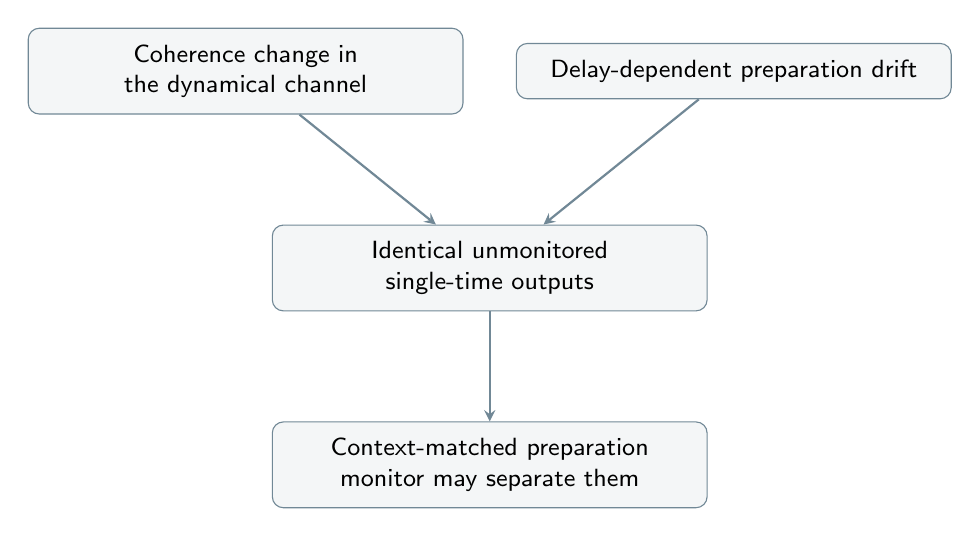
\begin{tikzpicture}[>=stealth, every node/.style={draw=blue!65,rounded corners=4pt,fill=blue!5,align=center,text width=5.1cm,font=\small\sffamily,inner sep=6pt}]
\node (dynamic) at (-3.1,0) {Coherence change in the dynamical channel};
\node (preparation) at (3.1,0) {Delay-dependent preparation drift};
\node (same) at (0,-2.5) {Identical unmonitored single-time outputs};
\node (monitor) at (0,-5.0) {Context-matched preparation monitor may separate them};
\draw[->,thick,blue!65] (dynamic) -- (same);
\draw[->,thick,blue!65] (preparation) -- (same);
\draw[->,thick,blue!65] (same) -- (monitor);
\end{tikzpicture}
\caption{Two physically admissible explanations can produce the same unmonitored outputs. A preparation monitor distinguishes this constructed pair only when its calibration transfers to the delayed experiment. The arrows summarize the conditional identifiability argument, not experimental observations.}
\end{figure}

\section{A calibrated rejection rule and the independent sampling unit}
A calibrated contrast increase can reject the entire nonincreasing-coherence null, rather than merely a particular exponential fit, but its error guarantee depends on what constitutes an independent observation. For the stipulated invertible, positive-real, fixed-axis dephasing model, let $g_i=g(i)$ denote the dimensionless coherence multiplier at each of two prespecified elapsed times $s<t$. The completely positive (CP)-divisible null requires $0<g_t\leq g_s\leq1$. The statistical task is therefore to distinguish a system-coherence increase from changes in preparation and readout contrast, while accounting separately for calibration uncertainty and sampling fluctuations.

At each time $i\in\{s,t\}$, use two preparation labels $a\in\{-1,+1\}$ for matched antipodal transverse preparations. Acquire $n$ delayed outcomes $Y_{a,i,k}\in\{-1,+1\}$ per label and $m$ no-wait reference outcomes $R_{a,i,k}\in\{-1,+1\}$ per label, where $k$ indexes repetitions. Under exact calibration transfer, their means are $\mathbb E Y_{a,i,k}=b_i+a v_i g_i$ and $\mathbb E R_{a,i,k}=b_i+a v_i$, with nonnegative effective visibility $0\leq v_i\leq1$ and physical probability constraint $|b_i|+v_i\leq1$. The offset $b_i$ is common to the two preparation labels; the visibility includes any common transverse preparation amplitude only insofar as that amplitude transfers identically between reference and delayed measurements.

The reference preparations bypass the system\textquoteright{}s waiting evolution but must reproduce the relevant preparation, analysis-pulse, trigger, readout, and acquisition context. The shot-level result assumes independent outcomes, reference batches independent of delayed batches, and reproducible fixed-setting means rather than an unmodeled shared random effect. It also retains fresh, initially factorized preparations with a common preparation-independent environment distribution and the known dephasing axis. These are applicability premises, not properties established by acquiring reference shots; randomized interleaving alone proves neither calibration transfer nor acquisition independence.

First, preparation differencing removes the label-common offset from the mean signal. Writing bars for sample averages within a setting, define the delayed contrast and its reference counterpart by $\widehat C_i=(\overline Y_{+,i}-\overline Y_{-,i})/2$ and $\widehat v_i=(\overline R_{+,i}-\overline R_{-,i})/2$. Their expectations are $C_i=v_i g_i$ and $v_i$, respectively. Thus a common offset does not bias the contrast, although finite-sample fluctuations remain; label-dependent offsets are not covered by this cancellation.

Second, nonincreasing system coherence bounds the mean contrast increase by visibility drift. To expose this distinction, write $\Delta=C_t-C_s$ and $\eta=|v_t-v_s|$. Under the null, $\Delta=v_t(g_t-g_s)+(v_t-v_s)g_s\leq|v_t-v_s|=\eta$, because the first term is nonpositive and $g_s\leq1$. Consequently, a positive delayed contrast difference is not sufficient for rejection: it must exceed the increase that admissible apparatus drift can produce.

Third, reference concentration supplies an observable upper bound on that drift. For a chosen calibration failure budget $\zeta\in(0,1)$, define $\epsilon=\sqrt{\log(4/\zeta)/m}$. Each reference contrast is a sum of $2m$ independent weighted outcomes whose squared range lengths sum to $2/m$, giving $\Pr(|\widehat v_i-v_i|>\epsilon)\leq2\exp(-m\epsilon^2)$. A union bound over the two prespecified times therefore gives simultaneous coverage with probability at least $1-\zeta$.

On this reference-coverage event, the triangle inequality yields $\eta\leq U=|\widehat v_t-\widehat v_s|+2\epsilon\leq\eta+4\epsilon$. The quantity $U$ is therefore a conservative upper bound on visibility drift, not an estimate of system memory. Its construction uses the raw reference contrasts; replacing them by fitted or optimistically clipped values would require a separate coverage argument. This calibration allocation covers the specified pair, not an unrestricted search across additional times.

For the delayed measurements, define $\widehat\Delta=\widehat C_t-\widehat C_s$ and choose a one-sided failure budget $\alpha\in(0,1)$. The squared range lengths of the $4n$ weighted outcomes in this difference sum to $4/n$, so the independent bounded-outcome inequality gives $\Pr(\widehat\Delta-\Delta>q_\alpha)\leq\alpha$, where $q_\alpha=\sqrt{2\log(1/\alpha)/n}$. The resulting rejection rule is $\widehat C_t-\widehat C_s>|\widehat v_t-\widehat v_s|+2\epsilon+\sqrt{2\log(1/\alpha)/n}$. Under the null, rejection requires either failed reference coverage or an excessive upward delayed-data fluctuation; hence its probability is at most $\alpha+\zeta$.

This error budget separates two statistical costs: increasing $m$ tightens reference calibration, whereas increasing $n$ reduces delayed-data uncertainty. A deterministic transfer tolerance introduces a third, systematic cost. If the delayed and reference visibilities satisfy $|v_i^{D}-v_i^{R}|\leq e$ at both times, with all visibilities nonnegative, then the null permits $C_t-C_s\leq|v_t^{R}-v_s^{R}|+e(g_t+g_s)\leq|v_t^{R}-v_s^{R}|+2e$. Adding $2e$ to the rejection threshold preserves the same statistical error allocation. This allowance is sharp for the stated transfer-error class, including identity system evolution, and cannot be removed by increasing shot counts.

In contrast, dependence within a nominal batch can invalidate the shot-level concentration argument even when every individual outcome has the correct marginal mean. Consider a CP-divisible family that reaches coherence $g=1/2$ before both observation times and remains constant, with exactly known visibility $v=1$ and zero offset. At each preparation\textendash{}time setting, draw one outcome with the stipulated mean and copy it across all $n$ recorded shots, keeping the four setting-level draws independent. Each estimated contrast then takes values $1$, $0$, and $-1$ with probabilities $9/16$, $6/16$, and $1/16$, respectively, regardless of the recorded shot count.

The event that the early contrast is nonpositive and the late contrast equals one has probability $(7/16)(9/16)=63/256$. Once the nominal shot-based radius is below $1/2$, this event causes false rejection despite the constant system coherence. Its probability exceeds a nominal level of $0.05$ and does not decrease as more copies are recorded. The counterexample does not contradict the independent-shot theorem; it shows that the number of recorded outcomes cannot replace the number of independent random draws.

A proposed extension therefore takes an entire acquisition superblock as the independent unit. Each superblock contains delayed and no-wait reference subblocks for the preparation labels and observation times, allowing arbitrary dependence among outcomes, settings, and references inside it. For superblock $b$ and time $j$, define $Z_{bj}=(\overline Y_{+,bj}-\overline Y_{-,bj})/2$ and $R_{bj}=(\overline R_{+,bj}-\overline R_{-,bj})/2$; both remain in $[-1,1]$ irrespective of the number or dependence of their constituent shots. Independent acquisition vectors across superblocks then support bounded-variable concentration, with uncertainty governed by the number of independent superblocks rather than the number of repeated shots.

The block-level proof candidate combines simultaneous delayed and reference constraints with a prespecified transfer tolerance, and asks whether any nonincreasing positive coherence sequence remains feasible. Its logical error argument is that, on joint coverage, a true null supplies a feasible sequence; rejection by infeasibility can therefore occur only when coverage fails. It asserts a false-rejection bound of $\alpha+\beta$, where $\alpha$ and $\beta$ are the delayed and reference failure budgets, but remains unresolved as a fully specified rejection procedure because the complete interval definitions and boundary rules are not available. No numerical power benchmark is adopted from that proposal.

The established rejection criterion thus turns an apparent revival into an exclusion of the restricted CP-divisible null only when both calibration transfer and the independent sampling unit are defensible. Its confidence comes from independent information, not from the length of an acquisition record: copied outcomes provide a concrete case in which an increasingly narrow nominal threshold becomes increasingly misleading.

\section{What additional regularity permits between samples}
An independently justified bound on rate variation permits finite coherence measurements to certify CP divisibility between sampling times, rather than merely fail to detect a revival. Retain the fixed-axis, positive-real dephasing model: the dimensionless coherence multiplier satisfies $g(0)=1$ and $0<g(t)\leq1$ on the observation window $0\leq t\leq T$. Define the local decay rate by $\kappa(t)=-d\log g(t)/dt$, and impose the additional assumption $|\kappa(t)-\kappa(s)|\leq K|t-s|$ throughout that window, with an externally supplied constant $K\geq0$.

Time has physical time units, $\kappa$ has inverse-time units, and $K$ has inverse-time-squared units; a continuously differentiable rate satisfying $|\kappa'(t)|\leq K$ is sufficient, but differentiability without a numerical bound is not the required premise.

The interpolation argument bounds how far an instantaneous rate can lie below its interval average. Fix sampling times $0=t_0<t_1<\cdots<t_m=T$, and define the interval length $h_i=t_{i+1}-t_i$ and average rate $\overline\kappa_i=h_i^{-1}\int_{t_i}^{t_{i+1}}\kappa(s)\,ds$. For any fixed $t\in[t_i,t_{i+1}]$, Lipschitz continuity gives $\kappa(t)\geq\kappa(s)-K|t-s|$ for every $s$ in the same interval. Integrating this comparison over $s$ yields
$\kappa(t)\geq\overline\kappa_i-Kd_i(t),\qquad d_i(t)=\frac{(t-t_i)^2+(t_{i+1}-t)^2}{2h_i}.$

The quantity $d_i(t)$ is the mean distance from $t$ to points in its sampling interval. It equals $h_i/4$ at the midpoint and reaches $h_i/2$ at either endpoint, so the interval-wide lower bound is
$\kappa(t)\geq\overline\kappa_i-\frac{Kh_i}{2}.$
The endpoint value, rather than the smaller midpoint value, is needed to protect the entire interval. Reversing the Lipschitz comparison also gives $\kappa(t)\leq\overline\kappa_i+Kd_i(t)$, allowing confidence bounds on the average to be propagated into a pointwise rate band.

The measured quantities enter through simultaneous bounds on endpoint coherences, not through derivatives of a fitted decay curve. Let $[L_i,U_i]$ be calibrated intervals for $g_i=g(t_i)$, and let $\mathcal E$ denote the event that every endpoint is covered. Under the independent bounded-outcome acquisition and transferable calibration assumptions, allocate a sampling-error budget $\alpha_s$ and a calibration-noncoverage budget $\beta$ so that $\Pr(\mathcal E)\geq1-\alpha_s-\beta$. The intervals may share data or endpoints: the propagation below requires simultaneous coverage, not independence between the intervals.

Positive endpoint bounds yield interval-average rate bounds because integrating the definition of the local rate gives
$\overline\kappa_i=\frac{\log g_i-\log g_{i+1}}{h_i}.$
The logarithmic ratio increases with its numerator and decreases with its denominator. Consequently, on $\mathcal E$,
$A_i^-\leq\overline\kappa_i\leq A_i^+,\qquad A_i^-=\frac{\log L_i-\log U_{i+1}}{h_i},\qquad A_i^+=\frac{\log U_i-\log L_{i+1}}{h_i}.$
These bounds remain simultaneous across all sampling intervals, despite their shared endpoints.

Positivity is consequential here, rather than a numerical convenience. Finite logarithmic bounds require the corresponding lower endpoints to be strictly positive; a zero lower endpoint is handled by the extended convention $\log0=-\infty$, leaving the affected rate bound uninformative. It must not be replaced by an arbitrary positive floor to obtain a certificate. An empty interval with $L_i>U_i$, or one with $U_i\leq0$, instead signals incompatibility with the assumed positive-dephasing and calibration description.

Combining statistical coverage with deterministic interpolation gives the simultaneous pointwise band
$A_i^- - Kd_i(t)\leq\kappa(t)\leq A_i^+ + Kd_i(t).$
A sufficient whole-window certification rule is therefore
$A_i^-\geq\frac{Kh_i}{2}\quad\text{for every }i=0,\ldots,m-1.$
On $\mathcal E$, this margin makes $\kappa(t)$ nonnegative at every observed and unobserved time in the window. For the stipulated invertible dephasing family, the intermediate map from $s$ to $t$ multiplies coherence by $g(t)/g(s)=\exp[-\int_s^t\kappa(u)\,du]$; nonnegative rates keep this multiplier at most one, establishing complete positivity and trace preservation of every intermediate map.

The error guarantee follows directly from that implication. For any fixed non-CP-divisible trajectory satisfying the model and regularity premises, a whole-window certificate can be reported only outside $\mathcal E$, so its false-certification probability is at most $\alpha_s+\beta$. This is a frequentist error bound, not a posterior probability that the dynamics are Markovian. If the supplied bound on $K$ itself has a nonzero confidence-failure probability, that probability must also enter the error budget. Failure to meet the margin is inconclusive: a sufficient certificate need not hold for every genuinely CP-divisible trajectory.

A physical counterexample shows why a finite regularity bound and nonnegative average rate cannot replace the margin. For $K>0$ and $0\leq t\leq h$, consider
$g(t)=\exp\!\left[-\frac{K}{2}t(h-t)\right],\qquad\kappa(t)=K\left(\frac h2-t\right).$
Because $t(h-t)\geq0$, the coherence remains in $0<g(t)\leq1$, so every map is an invertible, completely positive and trace-preserving dephasing channel. Nevertheless, the rate is $K$-Lipschitz and negative for $t>h/2$, while its interval average is zero and both endpoint channels are the identity. Exact endpoint agreement thus conceals an interval of coherence recovery even when the finite rate-variation bound is known.

The certificate remains conditional on physical premises not established by these endpoint contrasts. No independent experimental validation is supplied for the positive-real fixed-axis model, matched preparations and preparation-label symmetry, calibration transfer, independent acquisition units, or a numerical physical bound on $K$; the assumed reproducible, input-independent environmental preparation likewise cannot be inferred from those contrasts. In particular, selecting a convenient $K$ from the same fitted trajectory does not supply the external restriction used in the proof.

The resulting distinction is precise: the observations bound integrated decay, while an independently justified $K$, together with the margin $A_i^-\geq Kh_i/2$, excludes hidden negative-rate excursions throughout each sampling gap.

\section{Prospective predictive comparison and its support requirement}
Predictive comparison adds a distinct requirement to calibrated rejection of completely positive (CP)-divisible dephasing: a fitted explanation must assign meaningful probabilities to observations not used in fitting. The proposed synthetic study compares semigroup dynamics, a revival-capable dephasing family, and semigroup dynamics combined with preparation or readout variation. Its performance remains unmeasured; the substantive result developed here is an analytical support defect in the proposed predictive likelihood and a conditional repair, not a numerical ranking of these explanations. [C32\textendash{}C34]

The comparison is designed to separate dynamical modulation from apparatus modulation rather than to reward a more flexible decay curve alone. Calibration observations enter alongside delayed measurements, so uncertainty in preparation and readout is part of the inference rather than an exact correction imposed before fitting. The proposed primary acquisition model uses independent binomial counts, prespecified training and held-out times, physically constrained finite-grid likelihood fitting, and a finite-model complexity penalty. Selecting the revival-capable family would still require a separate divisibility classification: its fitted parameter space includes divisible as well as indivisible dynamics.

The controls address two different ways in which predictive attribution can fail. Deliberately failed calibration transfer retains cases where an apparatus-confounded semigroup and the dynamical alternative have identical complete observation likelihoods; such cases test attribution errors rather than discrimination between distinguishable models. Dependent-acquisition controls instead change the sampling law by allowing repeated shots to share an outcome. These controls must be reported separately from the primary independent-count comparison, because successful performance under the latter does not establish robustness to either failure.

The corrected primary factorial size is $3\times2\times2\times2\times3\times3=216$ conditions. At $2{,}000$ replicates per condition, this gives $432{,}000$ primary datasets, not the count implied by the earlier total of $648$ conditions. The earlier interval failure allocation of $0.05/648$ remains conservative for the corrected set of $216$ primary rejection proportions. Planned outcomes include predictive scores, false-positive frequencies, power, coverage, robustness, and model-attribution errors, none of which has been measured.

A consequential specification limit remains: the complete numerical grids, nuisance trajectories, calibration allocation, training and held-out schedules, fitting and failure rules, and penalty values are not all reproduced in the available description. Those values must be restored before the design can serve as an executable preregistration; they cannot be inferred from the factorial total or replaced by newly chosen values without identifying a design change. In particular, a conditional analytical power bound is not an estimate of the implemented procedure\textquoteright{}s power, and it does not supply the missing predictive comparison.

The dependence-aware extension exposes a further issue that must be resolved before execution. Here an acquisition block contains eight count cells: delayed and no-wait reference measurements, each with two antipodal preparation labels, at each of two times. Let $n>1$ be the number of binary shots per cell, let $p_c$ be the success probability in cell $c$, and let $d\in[0,1]$ be the copied-outcome mixture weight. With probability $1-d$, shots are generated independently; with probability $d$, one Bernoulli outcome is drawn independently for each cell and copied throughout that cell. This mixture preserves the cell-level success probabilities while changing the distribution of counts.

To see the support defect, consider a training block in which every count is an endpoint, either $0$ or $n$. For each cell, define $u_c=p_c$ when its observed count is $n$ and $u_c=1-p_c$ when it is $0$, and write $E=\prod_{c=1}^{8}u_c$. When the cell probabilities are interior, $0<E<1$, and the likelihood of this endpoint block is $L(d)=(1-d)E^n+dE$. Because $n>1$ implies $E^n<E$, this likelihood increases strictly with $d$. An all-endpoint training record therefore permits a maximum-likelihood fit at $d=1$, even though that record has positive probability under a true model with $d<1$.

At the fitted boundary $d=1$, every cell count must be an endpoint. An independent held-out block containing an interior count consequently receives fitted probability zero, although such a block has positive probability under a true model with $d<1$ and interior cell probabilities. Its log score is then $-\infty$; if two fitted candidates both assign zero probability, their log-score difference is undefined. Thus the proposed unconditional mean log-score differences and their standard errors are not generally well-defined. This is a counterexample to the scoring protocol, not to the physical dephasing models or the calibrated rejection witness.

A prespecified full-support predictive mixture repairs this particular failure. Let $P_{\mathrm{fit}}$ denote the fitted probability law for an eight-cell block, let $\lambda$ be a fixed smoothing weight with $0<\lambda\leq1$, and let $Q$ be the product of eight $\operatorname{Binomial}(n,1/2)$ count laws. Define the predictive distribution by $\widetilde P=(1-\lambda)P_{\mathrm{fit}}+\lambda Q$. The reference law supplies positive probability to every possible count vector, including outcomes excluded by a boundary fit.

The resulting score bound follows directly from the count probabilities. For a block count vector $\mathbf{k}=(k_1,\ldots,k_8)$ with each $k_c\in\{0,\ldots,n\}$, the reference probability is $Q(\mathbf{k})=\prod_{c=1}^{8}\binom{n}{k_c}2^{-n}\geq2^{-8n}$. Consequently $\widetilde P(\mathbf{k})\geq\lambda2^{-8n}$, and its natural-log score satisfies $\log\widetilde P(\mathbf{k})\geq\log\lambda-8n\log2$. For fixed $n$ and positive fixed $\lambda$, this prevents the zero-support counterexample and makes the block log score finite. It establishes a property of the proposed predictive distribution, not evidence of improved discrimination.

The repair also changes what is being compared: held-out scores would evaluate the smoothed predictive laws rather than the unsmoothed maximum-likelihood fits. The smoothing weight and its sensitivity analysis therefore remain to be fixed, together with the score estimand and the associated complexity comparison; the reference-withheld analysis also needs an explicit support-preserving specification. Predictive evidence can complement the calibrated rejection argument only after these choices make the comparison mathematically well-defined. Better fitting alone cannot supply that requirement, and repairing predictive support does not alter the assumptions needed to reject the CP-divisible null. [C32\textendash{}C34]

\section{Operational interpretation and validation limits}
A calibrated coherence increase can exclude the stipulated completely positive (CP)-divisible dephasing null, but it cannot by itself select a unique dynamical model or identify an environmental mechanism. The relevant null comprises all nonincreasing positive-real coherence functions within the common, invertible, fixed-axis dephasing description, not merely exponential decay. Consequently, rejecting this null is stronger than finding that a revival model fits better than a semigroup, yet narrower than rejecting every CP-divisible qubit evolution.

The statistical content of that exclusion is conditional and explicit. For the prespecified pair of observation times, the contrast-increase rule bounds false rejection by $\alpha+\zeta$, where $\alpha$ is the delayed-data tail-probability allowance and $\zeta$ is the simultaneous reference-calibration failure allowance. Preparation-label-common offsets cancel in the contrast difference, while transferable nonnegative reference contrast bounds the increase that visibility drift could produce under the null.

An increase exceeding both that allowance and the finite-sampling threshold is therefore incompatible with the restricted null at the stated error budget; this is an analytical guarantee, not an observed rejection frequency or a probability that the null is true.

Physical interpretation requires separate evidence for the assumptions connecting measured contrast to system coherence. Fresh preparations must be initially uncorrelated with a common, preparation-independent environment distribution, and the controls must support a reproducible fixed-axis description in a known frame. Matched preparations, preparation-label symmetry, and reference-to-delayed calibration transfer must also be independently defensible.

These properties have not been experimentally established here: for example, an increase in one transverse component can arise from coherent rotation rather than increased state-pair distinguishability, so calibrated quadrature measurements or fuller channel characterization are needed before extending the inference beyond real dephasing.

Calibration and acquisition assumptions are consequential rather than merely technical. The apparatus countermodels show that failed transfer can preserve the complete reference-plus-delayed likelihood of an apparent dynamical revival while the reduced system remains a semigroup; more shots from that protocol cannot resolve an exact observational equivalence. Likewise, the copied-shot construction shows why the independent-shot guarantee does not survive arbitrary within-setting dependence.

Randomized interleaving and no-wait references can challenge particular confounders, but do not establish transfer or independence by themselves; if dependence remains, the acquisition unit and concentration argument must be justified for that dependence structure.

The operational meaning of a successful rejection is correspondingly restricted. In positive-real scalar dephasing, increasing coherence also increases the trace distance of the fixed pair of ideal antipodal transverse preparations, so CP indivisibility and this information-backflow witness coincide within the selected family. That restricted agreement does not turn either diagnostic into a process-tensor memory test. Nor does it distinguish a quantum environment from classical colored noise: the latter is a possible mechanism for reduced dynamics, not an operational category mutually exclusive with CP indivisibility.

A process-memory investigation would instead require intervention-conditioned records testing whether future outcomes retain dependence on the earlier history after an appropriate causal break. Such an investigation needs independently validated resets and quantified reset errors, control cross-talk, and apparatus memory before residual dependence can be attributed to the system\textendash{}environment process. Controlled-model discrimination, including an echo comparison, addresses a different question unless its intervention-conditioned statistics and causal-break assumptions support the stronger claim. No such empirical process-tensor evidence has been obtained here.

The remaining validation limits concern distinct extensions of the argument. Failure to reject at sampled times does not certify continuous-time divisibility; a between-sample certificate additionally requires an independently defensible physical rate-regularity bound, which is not supplied for an apparatus. Predictive performance and implementation robustness remain unmeasured because the synthetic comparison has not been executed, and its identified predictive-support defect requires repair before the proposed score summaries can be used.

Agreement with published criteria and novelty are also unassessed because the identified primary research texts and relevant identifiability and state-preparation-and-measurement literature were not inspected.

The resulting evidential boundary separates exclusion from attribution. When the dynamical model, calibration transfer, and independent acquisition units are independently supported, the calibrated increase can rule out every CP-divisible explanation inside the stipulated dephasing class without privileging one revival ansatz. When those premises remain open, the same records constrain a joint system-and-apparatus explanation instead. Further physical attribution then requires measurements that test those premises or intervention-conditioned hypotheses, rather than simply increasing the number of observations made under the same assumptions.

\section{Limitations}
\begin{itemize}
\item The conclusions apply to positive-real, invertible, fixed-axis dephasing with a common preparation-independent channel. A transverse contrast revival does not by itself reject arbitrary CP-divisible qubit dynamics.
\item Preparation and readout transfer are external premises. Exact confounder equivalences show that additional shots and held-out prediction cannot resolve some violations.
\item The bounded index supports selected analytical steps but not exhaustive proof-level review. The finite-gap theorem, complete block confidence construction, and numerical sharp transfer boundary retain unresolved status.
\item No experimental data or executed simulations support performance claims. Analytical coverage or power statements must not be described as measured rejection rates or predictive accuracy.
\item Process-tensor memory and uniquely quantum microscopic mechanisms are outside the established conclusions. The complete reported classical-noise and control-response derivations are not available in the preview.
\item Primary research texts were not inspected, so the article cannot claim literature novelty or completed benchmarking against published criteria.
\item Saved research session [Research session 1] ended with an incomplete review; call 18 (skeptic) was not successfully completed. Earlier findings remain available, but this process limitation prevents claiming that the planned adversarial review was fully performed.
\end{itemize}
\section{Open obligations}
\begin{itemize}
\item Retrieve the complete finite-gap construction, including parameter choices, patch boundaries, and the fourth-power sine regularity repair, before presenting a fully reviewed proof.
\item Retrieve the complete block-level measurement model, interval formulas, feasible-set rule, and power calculation; check that all concentration bounds use independent superblocks rather than repeated shots.
\item Obtain the exact two-time benchmark means and compatibility derivation underlying the reported $q^*\approx0.0765$ threshold. Sharp compatibility for the full time schedule, extra calibrated quadratures, and a semigroup-only null remains unresolved.
\item Retrieve all omitted synthetic-study grids, nuisance trajectories, calibration allocations, train/test schedules, fitting rules, penalties, and failure-reporting conventions before implementation.
\item Fix the predictive smoothing weight and sensitivity analysis before executing the repaired comparison. Measure false-positive frequency, power, coverage, held-out prediction, fitting sensitivity, and model-attribution errors with reproducible outputs.
\item Independently characterize the dephasing axis, matched preparation contexts, label symmetry, calibration-transfer tolerances, and independent acquisition unit before applying the guarantees experimentally.
\item Obtain an independently defensible physical rate-regularity bound before claiming between-sample certification; endpoint observations cannot supply that premise themselves.
\item Inspect the primary texts identified by DOI 10.1103/PhysRevLett.103.210401, DOI 10.1103/PhysRevLett.105.050403, and DOI 10.1103/PhysRevLett.120.040405, together with relevant identifiability and SPAM literature, before assessing prior art or novelty.
\item Obtain intervention-conditioned records and independently validated causal breaks or resets before making empirical process-tensor memory claims.
\end{itemize}
\section{Conclusions}
Finite noisy observations can justify rejecting the stipulated CP-divisible dephasing null when a prespecified coherence-increase statistic exceeds independently calibrated statistical and systematic allowances. This is a conditional frequentist decision, not a probability that the environment possesses quantum memory.

Exact preparation and readout alternatives show why apparent revival and improved fitting are insufficient. The copied-shot counterexample further shows that confidence depends on independent information, not nominal repetition count.

Between-sample certification requires an additional quantitative regularity premise and a rate margin; otherwise endpoint agreement can conceal recovery. The unrestricted finite-schedule theorem remains a proof candidate pending complete review.

The defensible outcome is a bounded theoretical account and a prospective evaluation design, not an executed computational study, a verified physical memory effect, or a novelty claim.

\section*{Claim and source notes}
These notes identify the saved evidence for claims used in the article. The complete claim register and reasoning are retained in the paper record.
\begin{sloppypar}
\small
\begin{description}
\item[C19] The model describes longitudinal pure dephasing in a known rotating frame and excludes energy relaxation; its applicability requires fresh, initially factorized preparations, a preparation-independent environment distribution, reproducible controls, and a common channel at each delay. \textit{Status: }established.
\textit{Evidence: }[Research session 1, artifact 7], [Research session 1, artifact 2]
\item[C20] For a real coherence multiplier satisfying $g(0)=1$ and $0<g(t)\leq1$, the dephasing channel is CPTP and invertible. It is CP divisible exactly when $g$ is nonincreasing, equivalently when the continuous local rate $\kappa(t)=-d\log g(t)/dt$ is nonnegative; the ideal antipodal transverse pair has trace distance $g(t)$. \textit{Status: }established.
\textit{Evidence: }[Research session 1, artifact 1], [Research session 1, artifact 2]
\item[C21] A valid semigroup baseline is $g_M(u)=e^{-\lambda u}$, with $u=t/\Delta$ and $\lambda\geq0$. The candidate $g_N(u)=e^{-\lambda u}[1-a\sin^2(\pi u)]$ is CPTP and invertible for $0\leq a<1$; at $\lambda=1$ and $a=1/2$, it increases between $u=1/2$ and $u=1$ by $e^{-1}-e^{-1/2}/2>0$. Time dependence alone is insufficient: $g(t)=e^{-\gamma t-bt^2}$ has nonnegative rate for $\gamma,b\geq0$. \textit{Status: }established.
\textit{Evidence: }[Research session 1, artifact 6], [Research session 1, artifact 4]
\item[C22] The saved proof candidate asserts that every finite single-time sampling schedule with a nonzero gap admits an invertible, non-CP-divisible dephasing family agreeing exactly with a dephasing semigroup at all sampled times, hence producing identical single-time tomography likelihoods. \textit{Status: }unresolved.
\textit{Evidence: }[Research session 1, artifact 1], [Research session 1, artifact 2], [Research session 1]
\item[C23] Without independent preparation information, physical revival dynamics and semigroup dynamics preceded by delay-labelled preparation dephasing can have identical single-time likelihoods. For $c_a(u)=1-a\sin^2(\pi u/2)$, dynamics $e^{-ru}c_a(u)$ with fixed preparation and dynamics $e^{-ru}$ with preparation contrast $c_a(u)$ produce the same outputs. \textit{Status: }established.
\textit{Evidence: }[Research session 1, artifact 5]
\item[C24] Calibration-transfer uncertainty creates a systematic ambiguity that cannot be removed by increasing shots. If each delayed visibility differs from its reference by at most $e$, an additional $2e$ allowance in a two-time contrast-increase threshold is sharp for that transfer-error class. \textit{Status: }established.
\textit{Evidence: }[Research session 1, artifact 6], [Research session 1, artifact 5]
\item[C25] A reported sharp two-time compatibility boundary occurs near transfer radius $q^*\approx0.0765$: below it the benchmark excludes the stipulated CP-divisible class, whereas at or above it a CP-divisible countermodel reportedly matches the exact mean records. \textit{Status: }unresolved.
\textit{Evidence: }[Research session 1]
\item[C26] Under independent shots, nonnegative transferable reference contrast, preparation-label-common offsets, and the positive-real dephasing model, reject the CP-divisible null when $\widehat C_t-\widehat C_s>|\widehat v_t-\widehat v_s|+2\epsilon+\sqrt{2\log(1/\alpha)/n}$, where $\epsilon=\sqrt{\log(4/\zeta)/m}$. With $n$ delayed shots and $m$ reference shots per preparation at each time, false rejection is at most $\alpha+\zeta$. \textit{Status: }established.
\textit{Evidence: }[Research session 1, artifact 6], [Research session 1, artifact 3]
\item[C27] The independent-shot guarantee can fail under copied outcomes even when each shot has the correct marginal mean. For a CP-divisible family with coherence $1/2$ at both observation times, the supplied construction yields a false-rejection event of probability $63/256$ once the nominal radius is below $1/2$. \textit{Status: }established.
\textit{Evidence: }[Research session 1, artifact 4], [Research session 1, artifact 7]
\item[C28] The saved block-level proof candidate replaces independent shots by independent acquisition superblocks and allows arbitrary dependence within a superblock. It asserts false rejection at most $\alpha+\beta$ for a calibrated feasible-set test of nonincreasing positive coherence. \textit{Status: }unresolved.
\textit{Evidence: }[Research session 1, artifact 7]
\item[C29] If the local rate is $K$-Lipschitz and valid simultaneous positive coherence intervals are available, interval-average rate bounds can certify CP divisibility throughout the observation window. On an interval of length $h_i$, the sufficient condition is $A_i^-\geq Kh_i/2$, where $A_i^-$ lower-bounds the average rate. \textit{Status: }established.
\textit{Evidence: }[Research session 1, artifact 2], [Research session 1, artifact 1]
\item[C30] A known finite regularity bound and nonnegative average rates do not suffice without the margin. For $K>0$ on $0\leq t\leq h$, the channel $g(t)=\exp[-Kt(h-t)/2]$ has identity endpoint channels but negative local rate near the final endpoint. \textit{Status: }established.
\textit{Evidence: }[Research session 1, artifact 2]
\item[C31] The supported reduced-map conclusions do not establish process-tensor memory or a uniquely quantum microscopic environment. Classical colored noise is a possible mechanism rather than an operational category excluding CP-indivisible reduced dynamics. \textit{Status: }limitation.
\textit{Evidence: }[Research session 1, artifact 1], [Research session 1, artifact 4], [Research session 1, artifact 7]
\item[C32] The synthetic predictive comparison is prospective, not an observed result. The corrected primary factorial count is $216$ conditions, giving $432{,}000$ datasets at $2{,}000$ replicates per condition; predictive performance, rejection frequencies, coverage, robustness, and attribution errors remain unmeasured. \textit{Status: }limitation.
\textit{Evidence: }[Research session 1], [Research session 1, artifact 6], [Research session 1, artifact 5]
\item[C33] The proposed dependence-mixture maximum-likelihood protocol can assign zero probability to possible held-out data, making unconditional mean log-score differences and their standard errors undefined. \textit{Status: }established.
\textit{Evidence: }[Research session 1, artifact 7]
\item[C34] A prespecified full-support predictive mixture would repair that support failure: $\widetilde P=(1-\lambda)P_{\mathrm{fit}}+\lambda Q$, with fixed $0<\lambda\leq1$ and $Q$ the product of eight $\operatorname{Binomial}(n,1/2)$ count laws, yields block log score at least $\log\lambda-8n\log2$. \textit{Status: }established.
\textit{Evidence: }[Research session 1, artifact 7]
\item[C35] Published-criteria agreement and novelty are unassessed because the identified primary texts and relevant identifiability and SPAM literature were not inspected. \textit{Status: }limitation.
\textit{Evidence: }[Research session 1], [Research session 1, artifact 4], [Research session 1, artifact 6]
\item[C36] Experimental applicability remains unestablished: fixed-axis real dephasing, matched preparations, label symmetry, calibration transfer, valid independent acquisition units, and a physical regularity bound have not been independently validated. \textit{Status: }limitation.
\textit{Evidence: }[Research session 1], [Research session 1, artifact 2], [Research session 1, artifact 6]
\end{description}
\end{sloppypar}
\section*{Paper writing source material used}
These sources informed manuscript organization and writing methods, not the scientific evidence or findings.
\begin{itemize}
\item IOP \textemdash{} Writing Your Journal Article (discipline): \url{https://publishingsupport.iopscience.iop.org/publishing-support/authors/authoring-for-journals/writing-journal-article/}
\item PLOS ONE \textemdash{} Manuscript and Reporting Guidelines (general): \url{https://journals.plos.org/plosone/s/submission-guidelines}
\item EASE \textemdash{} Guidelines for Authors of Scientific Articles (full text) (general): \url{https://pmc.ncbi.nlm.nih.gov/articles/PMC4130677/}
\end{itemize}
\end{document}
